\chapter{Specifikacija programske potpore}
		
	\section{Funkcionalni zahtjevi}
			
			\noindent \textbf{Dionici:}
			
			\begin{packed_enum}
				
				\item Naručitelji
				\item Učenici (korisnici)
				\item Administratori				
				\item Razvojni tim
				
			\end{packed_enum}
			
			\noindent \textbf{Aktori i njihovi funkcionalni zahtjevi:}
			
			
			\begin{packed_enum}
				\item  \underbar{Neregistrirani učenik (inicijator) može:}
				
				\begin{packed_enum}
					
					\item se registrirati e-mail adresom
					
				\end{packed_enum}
			
			
				\item  \underbar{Učenik (inicijator) može:}
				
				\begin{packed_enum}
					\item izvršiti prijavu u sustav za koju su mu potrebni e-mail adresa i lozinka
					\item promijeniti trenutnu lozinku
					\item obrisati svoj korisnički račun
					\item pregledavati postojeće rječnike grupirane po jeziku
					\item pokrenuti učenje riječi odabirom jednog od ponuđenih rječnika i načina učenja
					\item odgovarati na pitanja o riječima ovisno o odabranom načinu učenja
					
					\begin{packed_enum}
						\item odabirom točnog odgovora
						\item upisivanjem točnog odgovora
						\item snimanjem izgovora riječi u zvučnu datoteku
					\end{packed_enum}
					
				\end{packed_enum}
			
					
			\item  \underbar{Administrator (inicijator) može:}
			
			\begin{packed_enum}
				
				\item stvarati nove rječnike
				\item dodavati i brisati riječi iz rječnika
				\item uređivati komponente postojećih riječi u rječniku\newline
				
			\end{packed_enum}
			
			
			\item  \underbar{Korijenski administrator (inicijator) može:}
			
			\begin{packed_enum}
				
				\item definirati administratore
				\item stvarati nove rječnike
				\item dodavati i brisati riječi iz rječnika
				\item uređivati komponente postojećih riječi u rječniku
				
			\end{packed_enum}
		
			
			\item  \underbar{Baza podataka (sudionik):}
		
			\begin{packed_enum}
			
			\item pohranjuje rječnike
			\item pohranjuje sve podatke o učenicima i administratorima
			
			\end{packed_enum}
		
			
			\item  \underbar{Vanjski rječnik (sudionik):}
		
			\begin{packed_enum}
			
			\item sadrži informacije koje se koriste prilikom dodavanja novih riječi u rječnike
			
			\end{packed_enum}
		
			
			\item  \underbar{Servis za ocjenu kvalitete izgovora (sudionik):}
	
			\begin{packed_enum}
		
			\item provjerava točnost snimljene izgovorene riječi
			\item na temelju provjere odgovara s ocjenom u ljestvici od jedan do deset
		
			\end{packed_enum}		
		
	
			\end{packed_enum}
			
			\eject 
			
						
			\subsection{Obrasci uporabe}
					
				\subsubsection{Opis obrazaca uporabe}		

					\noindent \underbar{\textbf{UC1 - Registracija}}
					\begin{packed_item}
	
						\item \textbf{Glavni sudionik: }Učenik
						\item  \textbf{Cilj:} Stvoriti korisnički račun za pristup sustavu
						\item  \textbf{Sudionici:} Baza podataka
						\item  \textbf{Preduvjet:} -
						\item  \textbf{Opis osnovnog tijeka:}
						
						\item[] \begin{packed_enum}
	
							\item Učenik odabire gumb za registraciju
							\item Učenik unosi potrebne korisničke podatke
							\item Učenik prima obavijest o uspješnoj registraciji
						\end{packed_enum}
						
						\item  \textbf{Opis mogućih odstupanja:}
						
						\item[] \begin{packed_item}
	
							\item[2.a] Unos već zauzetog e-maila, unos već zauzetog korisničkog imena, unos neispravnog e-maila
							\item[] \begin{packed_enum}
								
								\item Sustav obavještava učenika o neuspjeloj registraciji i vraća ga natrag na stranicu za registraciju
								\item Učenik mijenja potrebne unesene podatke i završava unos ili odustaje od registracije
								
							\end{packed_enum}
							
						\end{packed_item}
					\end{packed_item}

					\noindent \underbar{\textbf{UC2 - Prijava u sustav}}
					\begin{packed_item}
	
						\item \textbf{Glavni sudionik: }Učenik
						\item  \textbf{Cilj:} Izvršiti prijavu u sustav
						\item  \textbf{Sudionici:} Baza podataka
						\item  \textbf{Preduvjet:} Registracija
						\item  \textbf{Opis osnovnog tijeka:}
						
						\item[] \begin{packed_enum}
	
							\item Unos korisničkog imena ili e-maila i lozinke
							\item Potvrda o ispravnosti unesenih podataka
							\item Pristup korisničkom sučelju
						\end{packed_enum}
						
						\item  \textbf{Opis mogućih odstupanja:}
						
						\item[] \begin{packed_item}
	
							\item[2.a] Neispravno uneseno korisničko ime, email ili lozinka
							\item[] \begin{packed_enum}
								
								\item Sustav obavještava učenika o neuspjeloj prijavi te ga vraća na stranicu za prijavu
								
							\end{packed_enum}
							
						\end{packed_item}
					\end{packed_item}

					\noindent \underbar{\textbf{UC3 - Pregled osobnih podataka}}
					\begin{packed_item}
	
						\item \textbf{Glavni sudionik: }Učenik
						\item  \textbf{Cilj:} Pregledati osobne podatke
						\item  \textbf{Sudionici:} Baza podataka
						\item  \textbf{Preduvjet:} Učenik je prijavljen u sustav
						\item  \textbf{Opis osnovnog tijeka:}
						
						\item[] \begin{packed_enum}
	
							\item Učenik odlazi na svoj profil
							\item Učenik odabire opciju "Osobni podatci"
							\item Aplikacije prikazuje osobne podatke učenika
						\end{packed_enum}
						
					\end{packed_item}

					\noindent \underbar{\textbf{UC4 - Promjena osobnih podataka}}
					\begin{packed_item}
	
						\item \textbf{Glavni sudionik: }Učenik
						\item  \textbf{Cilj:} Promijeniti osobne podatke
						\item  \textbf{Sudionici:} Baza podataka
						\item  \textbf{Preduvjet:} Učenik je prijavljen u sustav
						\item  \textbf{Opis osnovnog tijeka:}
						
						\item[] \begin{packed_enum}
	
							\item Učenik odlazi na svoj profil
							\item Učenik bira koje osobne podatke želi mijenjati
							\item Učenik mijenja odabrane osobne podatke
							\item Učenik sprema promjene
							\item Baza podataka ažurira napravljene promjene
						\end{packed_enum}
						
						\item  \textbf{Opis mogućih odstupanja:}
						
						\item[] \begin{packed_item}
	
							\item[4.a] Učenik mijenja svoje podatke, ali ne spremi promjene
							\item[] \begin{packed_enum}
								
								\item Sustav obavještava učenika da nije spremio podatke
								\item Učenik odabire želi li spremiti ili odbaciti napravljene promjene 
								
							\end{packed_enum}
							
						\end{packed_item}
					\end{packed_item}

					\noindent \underbar{\textbf{UC5 - Brisanje korisničkog računa}}
					\begin{packed_item}
	
						\item \textbf{Glavni sudionik: }Učenik
						\item  \textbf{Cilj:} Izbrisati svoj korisnički račun
						\item  \textbf{Sudionici:} Baza podataka
						\item  \textbf{Preduvjet:} Učenik je prijavljen u sustav
						\item  \textbf{Opis osnovnog tijeka:}
						
						\item[] \begin{packed_enum}
	
							\item Učenik odlazi na svoj profil
							\item Učenik bira opciju obriši korisnički račun
							\item Sustav ispituje učenika je li siguran da želi obrisati korisnički račun
							\item Učenik potvrđuje da želi obrisati korisnički račun
							\item Korisnički račun se briše iz baze podataka
							\item Sustav šalje učenika na stranicu za registraciju
						\end{packed_enum}
						
						\item  \textbf{Opis mogućih odstupanja:}
						
						\item[] \begin{packed_item}
	
							\item[4.a] Učenik ne potvrđuje brisanje računa, a izlazi iz aplikacije
							\item[] \begin{packed_enum}
								
								\item Sustav ne briše korisnički račun i obavještava učenika da korisnički račun nije obrisan
								
							\end{packed_enum}
							
						\end{packed_item}
					\end{packed_item}

					\noindent \underbar{\textbf{UC6 - Pregled rječnika}}
					\begin{packed_item}
	
						\item \textbf{Glavni sudionik: }Učenik
						\item  \textbf{Cilj:} Pregledati postojeće rječnike za učenje
						\item  \textbf{Sudionici:} Baza podataka
						\item  \textbf{Preduvjet:} Učenik je prijavljen u sustav
						\item  \textbf{Opis osnovnog tijeka:}
						
						\item[] \begin{packed_enum}
	
							\item Učenik odabire opciju "Pregled rječnika"
							\item Otvara se padajuća lista dostupnih jezika
							\item Učenik odabire jezik
							\item Otvara se stranica sa izborom rječnika koji su dostupni na odabranom jeziku
							\item Učenik odabire rječnik
							\item Otvara se stranica na kojoj učenik može pregledavati rječnik
						\end{packed_enum}
						
					\end{packed_item}

					\noindent \underbar{\textbf{UC7 - Pokretanje učenja}}
					\begin{packed_item}
	
						\item \textbf{Glavni sudionik: }Učenik
						\item  \textbf{Cilj:} Pokrenuti učenje jezika
						\item  \textbf{Sudionici:} Baza podataka
						\item  \textbf{Preduvjet:} Učenik je prijavljen u sustav
						\item  \textbf{Opis osnovnog tijeka:}
						
						\item[] \begin{packed_enum}
	
							\item Učenik bira opciju "Pokreni učenje"
							\item Otvara se padajuća lista jezika rječnika
							\item Učenik odabire jezik
							\item Otvara se stranica sa izborom rječnika koji dostupni na odabranom jeziku
							\item Učenik odabire rječnik iz kojeg želi učiti
							\item Otvara se stranica sa ponuđenim načinima učenja
							\item Učenik odabire način na koji želi učiti jezik
							\item Otvara se stranica na kojoj učenik odgovara na pitanja o riječima na temelju načina učenja kojeg je odabrao
						\end{packed_enum}
						
					\end{packed_item}

					\noindent \underbar{\textbf{UC8 - Prekid učenja}}
					\begin{packed_item}
	
						\item \textbf{Glavni sudionik: }Učenik
						\item  \textbf{Cilj:} Prekinuti učenje i spremiti napredak
						\item  \textbf{Sudionici:} Baza podataka
						\item  \textbf{Preduvjet:} Učenik je pokrenuo proces učenja
						\item  \textbf{Opis osnovnog tijeka:}
						
						\item[] \begin{packed_enum}
	
							\item Učenik bira opciju "Prekini učenje"
							\item Sustav učenika vraća na početnu stranicu aplikacije
						\end{packed_enum}
						
					\end{packed_item}

					\noindent \underbar{\textbf{UC9 - Promjena načina učenja}}
					\begin{packed_item}
	
						\item \textbf{Glavni sudionik: }Učenik
						\item  \textbf{Cilj:} Promijeniti način na koji učenik uči određeni jezik
						\item  \textbf{Sudionici:} Baza podataka
						\item  \textbf{Preduvjet:} Učenik je prijavljen u sustav
						\item  \textbf{Opis osnovnog tijeka:}
						
						\item[] \begin{packed_enum}
	
							\item Učenik bira opciju "Promijeni način učenja"
							\item Otvara se stranica sa jezicima
							\item Učenik odabire jezik koji trenutno uči
							\item Otvara se stranica sa izborom rječnika
							\item Učenik odabire rječnik iz kojeg trenutno uči
							\item Otvara se stranica sa ponuđenim načinima učenja
							\item Učenik odabire način na koji želi učiti jezik
							\item Baza podataka ažurira način učenja za određeni rječnik i jezik
						\end{packed_enum}
						
					\end{packed_item}

					\noindent \underbar{\textbf{UC10 - Učenje upitom riječi na odabranom jeziku uz odabir hrvatskog prijevoda}}
					\begin{packed_item}
	
						\item \textbf{Glavni sudionik: }Učenik
						\item  \textbf{Cilj:} Učiti prijevod riječi na hrvatski jezik
						\item  \textbf{Sudionici:} Baza podataka
						\item  \textbf{Preduvjet:} Učenik je pokrenuo proces učenja
						\item  \textbf{Opis osnovnog tijeka:}
						
						\item[] \begin{packed_enum}
	
							\item Učeniku se zadaje riječ iz odabranog rječnika i ponuđeni odgovori istoznačne hrvatske riječi
							\item Učenik odabire smatrani točan odgovor
							\item Učenik potvrđuje svoj odgovor
							\item Baza podataka ažurira podatke učenja učenika određenim rječnikom temeljeno na točnosti odgovora
							\item Ponavlja se prvi korak sve dok učenik ne prekine učenje
						\end{packed_enum}
						
					\end{packed_item}

					\noindent \underbar{\textbf{UC11 - Učenje upitom hrvatske riječi uz odabir prijevoda}}
					\begin{packed_item}
	
						\item \textbf{Glavni sudionik: }Učenik
						\item  \textbf{Cilj:} Učiti prijevod hrvatske riječi na odabrani jezik
						\item  \textbf{Sudionici:} Baza podataka
						\item  \textbf{Preduvjet:} Učenik je pokrenuo proces učenja
						\item  \textbf{Opis osnovnog tijeka:}
						
						\item[] \begin{packed_enum}
	
							\item Učeniku se zadaje hrvatska riječ iz odabranog rječnika i ponuđeni odgovori istoznačne riječi na odabranom jeziku
							\item Učenik odabire smatrani točan odgovor
							\item Učenik potvrđuje svoj odgovor
							\item Baza podataka ažurira podatke učenja učenika određenim rječnikom temeljeno na točnosti odgovora
							\item Ponavlja se prvi korak sve dok učenik ne prekine učenje
						\end{packed_enum}
						
					\end{packed_item}

					\noindent \underbar{\textbf{UC12 - Učenje upitom izgovora riječi na odabranom jeziku uz pisanje riječi}}
					\begin{packed_item}
	
						\item \textbf{Glavni sudionik: }Učenik
						\item  \textbf{Cilj:} Učiti točno pisanje riječi odabranog jezika na temelju izgovora
						\item  \textbf{Sudionici:} Baza podataka
						\item  \textbf{Preduvjet:} Učenik je pokrenuo proces učenja
						\item  \textbf{Opis osnovnog tijeka:}
						
						\item[] \begin{packed_enum}
	
							\item Učeniku se zadaje glasovni zapis riječi
							\item Učenik na obrazac upisuje izgovorenu riječ u tekstualnom obliku
							\item Učenik potvrđuje svoj odgovor
							\item Baza podataka ažurira podatke učenja učenika određenim rječnikom temeljeno na točnosti odgovora
							\item Ponavlja se prvi korak sve dok učenik ne prekine učenje
						\end{packed_enum}
						
					\end{packed_item}

					\noindent \underbar{\textbf{UC13 - Učenje upitom pisane riječi na odabranom jeziku uz snimanje izgovora}}
					\begin{packed_item}
	
						\item \textbf{Glavni sudionik: }Učenik
						\item  \textbf{Cilj:} Učiti izgovor riječi na temelju tekstualnog oblika riječi
						\item  \textbf{Sudionici:} Baza podataka, Servis za ocjenu kvalitete izgovora
						\item  \textbf{Preduvjet:} Učenik je pokrenuo proces učenja
						\item  \textbf{Opis osnovnog tijeka:}
						
						\item[] \begin{packed_enum}
	
							\item Učeniku se zadaje tekstualni zapis riječi
							\item Učenik odabire opciju za snimanje glasa
							\item Učenik u mikrofon izgovara zadanu riječ
							\item Učenik odabire opciju za prestanak snimanja glasa
							\item Učenik potvrđuje svoj odgovor
							\item Servis za ocjenu kvalitete izgovora ocjenjuje točnost izgovora riječi
							\item Baza podataka ažurira podatke učenja učenika određenim rječnikom temeljeno na točnosti odgovora
							\item Ponavlja se prvi korak sve dok učenik ne prekine učenje
						\end{packed_enum}

						\item  \textbf{Opis mogućih odstupanja:}
						
						\item[] \begin{packed_item}
	
							\item[2.a] Učenik nema detektirani mikrofon
							\item[] \begin{packed_enum}
								
								\item Sustav onemogućuje opciju snimanja glasa
								\item Sustav obavještava učenika nemogućnost snimanja glasa
								
							\end{packed_enum}
						\end{packed_item}
						
					\end{packed_item}

					\noindent \underbar{\textbf{UC14 - Dodavanje administratora}}
					\begin{packed_item}
	
						\item \textbf{Glavni sudionik: }Korijenski administrator
						\item  \textbf{Cilj:} Definirati nove administratore
						\item  \textbf{Sudionici:} Baza podataka
						\item  \textbf{Preduvjet:} Korisnik je prijavljen u sustav i dodijeljena su mu prava korijenskog administratora
						\item  \textbf{Opis osnovnog tijeka:}
						
						\item[] \begin{packed_enum}
	
							\item Korijenski administator odabire opciju postavljanja administratora
							\item Otvara se prozor za upis korisničkog imena korisnika
							\item Korijenski administrator upisuje korisničko ime i potvrđuje upis
							\item Baza podataka ažurira promjene za određeno korisničko ime
						\end{packed_enum}

						\item  \textbf{Opis mogućih odstupanja:}
						
						\item[] \begin{packed_item}
	
							\item[3.a] Upisano je neispravno korisničko ime
							\item[] \begin{packed_enum}
								
								\item Sustav obavještava korijenskog administratora o neuspjelom upisu
								
							\end{packed_enum}
						\end{packed_item}
						
					\end{packed_item}

					\noindent \underbar{\textbf{UC15 - Stvori rječnik}}
					\begin{packed_item}
	
						\item \textbf{Glavni sudionik: }Administrator
						\item  \textbf{Cilj:} Stvoriti novi rječnik
						\item  \textbf{Sudionici:} Baza podataka, Vanjski rječnik
						\item  \textbf{Preduvjet:} Korisnik je prijavljen u sustav i dodijeljena su mu prava administratora
						\item  \textbf{Opis osnovnog tijeka:}
						
						\item[] \begin{packed_enum}
	
							\item Administrator odabire opciju "Stvori novi rječnik"
							\item Administrator unosi riječi i podatke o novom rječniku
							\item Baza podataka ažurira novi rječnik
						\end{packed_enum}
						
					\end{packed_item}

					\noindent \underbar{\textbf{UC16 - Dodaj riječ}}
					\begin{packed_item}
	
						\item \textbf{Glavni sudionik: }Administrator
						\item  \textbf{Cilj:} Dodati riječ u postojeći rječnik
						\item  \textbf{Sudionici:} Baza podataka, Vanjski rječnik
						\item  \textbf{Preduvjet:} Korisnik je prijavljen u sustav i dodijeljena su mu prava administratora
						\item  \textbf{Opis osnovnog tijeka:}
						
						\item[] \begin{packed_enum}
	
							\item Administrator odabire opciju "Dodaj novu riječ"
							\item Otvara se prozor za odabir jezika i rječnika
							\item Administrator odabire jezik i rječnik u koji želi dodati novu riječ
							\item Otvara se prozor za upis riječi
							\item Administrator upisuje riječ
							\item Pokreće se procedura pretrage na vanjskom rječniku
							\item Administrator odabire opis i ostale podatke bitne za riječ koje je dobio od vanjskog rječnika
							\item Administrator uređuje odabrane podatke
							\item Administrator potvrđuje unos
							\item Baza podataka ažurira novu riječ za određeni jezik i rječnik
					
						\end{packed_enum}

						\item  \textbf{Opis mogućih odstupanja:}
						
						\item[] \begin{packed_item}
	
							\item[5.a] Upisana riječ već postoji u rječniku
							\item[] \begin{packed_enum}
								
								\item Sustav obavještava administratora o tome da upisana riječ već postoji u rječniku
								\item Administrator može odabrati opciju uređivanja postojeće riječi ili upisati drugu riječ
								
							\end{packed_enum}
						\end{packed_item}
						
					\end{packed_item}

					\noindent \underbar{\textbf{UC17 - Ukloni riječ}}
					\begin{packed_item}
	
						\item \textbf{Glavni sudionik: }Administrator
						\item  \textbf{Cilj:} Ukloniti riječ iz rječnika
						\item  \textbf{Sudionici:} Baza podataka
						\item  \textbf{Preduvjet:} Korisnik je prijavljen u sustav i dodijeljena su mu prava administratora
						\item  \textbf{Opis osnovnog tijeka:}
						
						\item[] \begin{packed_enum}
	
							\item Administrator odabire opciju "Ukloni riječ"
							\item Otvara se prozor za odabir jezika i rječnika
							\item Administrator odabire jezik i rječnik iz kojeg želi ukloniti riječ
							\item Otvara se prozor za upis riječi
							\item Administrator upisuje riječ
							\item Odabrana riječ se briše iz rječnika
						\end{packed_enum}

						\item  \textbf{Opis mogućih odstupanja:}
						
						\item[] \begin{packed_item}
	
							\item[5.a] Upisana riječ ne postoji
							\item[] \begin{packed_enum}
								
								\item Sustav obavještava administratora da upisana riječ ne postoji u rječniku
							\end{packed_enum}
						\end{packed_item}
						
					\end{packed_item}

					\noindent \underbar{\textbf{UC18 - Izmijeni riječ}}
					\begin{packed_item}
	
						\item \textbf{Glavni sudionik: }Administrator
						\item  \textbf{Cilj:} Izmijeniti riječ iz rječnika
						\item  \textbf{Sudionici:} Baza podataka
						\item  \textbf{Preduvjet:} Korisnik je prijavljen u sustav i dodijeljena su mu prava administratora
						\item  \textbf{Opis osnovnog tijeka:}
						
						\item[] \begin{packed_enum}
	
							\item Administrator odabire opciju "Izmijeni riječ"
							\item Otvara se prozor za odabir jezika i rječnika
							\item Administrator odabire jezik i rječnik u kojem želi izmijeniti riječ
							\item Otvara se prozor za upis riječi
							\item Administrator upisuje riječ
							\item Otvara se prozor za izmjenu opisa i podataka riječi
							\item Administrator mijenja opis riječi i podatke o riječi
							\item Administrator sprema promjene
							\item Baza podataka ažurira određenu riječ za određeni jezik i rječnik
						\end{packed_enum}

						\item  \textbf{Opis mogućih odstupanja:}
						
						\item[] \begin{packed_item}
	
							\item[5.a] Upisana riječ ne postoji
							\item[] \begin{packed_enum}
								
								\item Sustav obavještava administratora da upisana riječ ne postoji u rječniku
								
							\end{packed_enum}
							\item[8.a] Administrator nije spremio promjene
							\item[] \begin{packed_enum}
								
								\item Sustav obavještava administratora da nije spremio promjene
								\item Administrator odlučuje želi li spremiti ili odbaciti napravljene promjene
								
							\end{packed_enum}

						\end{packed_item}			
					\end{packed_item}
				
					
				\subsubsection{Dijagrami obrazaca uporabe}
					
					\begin{figure}[H]
						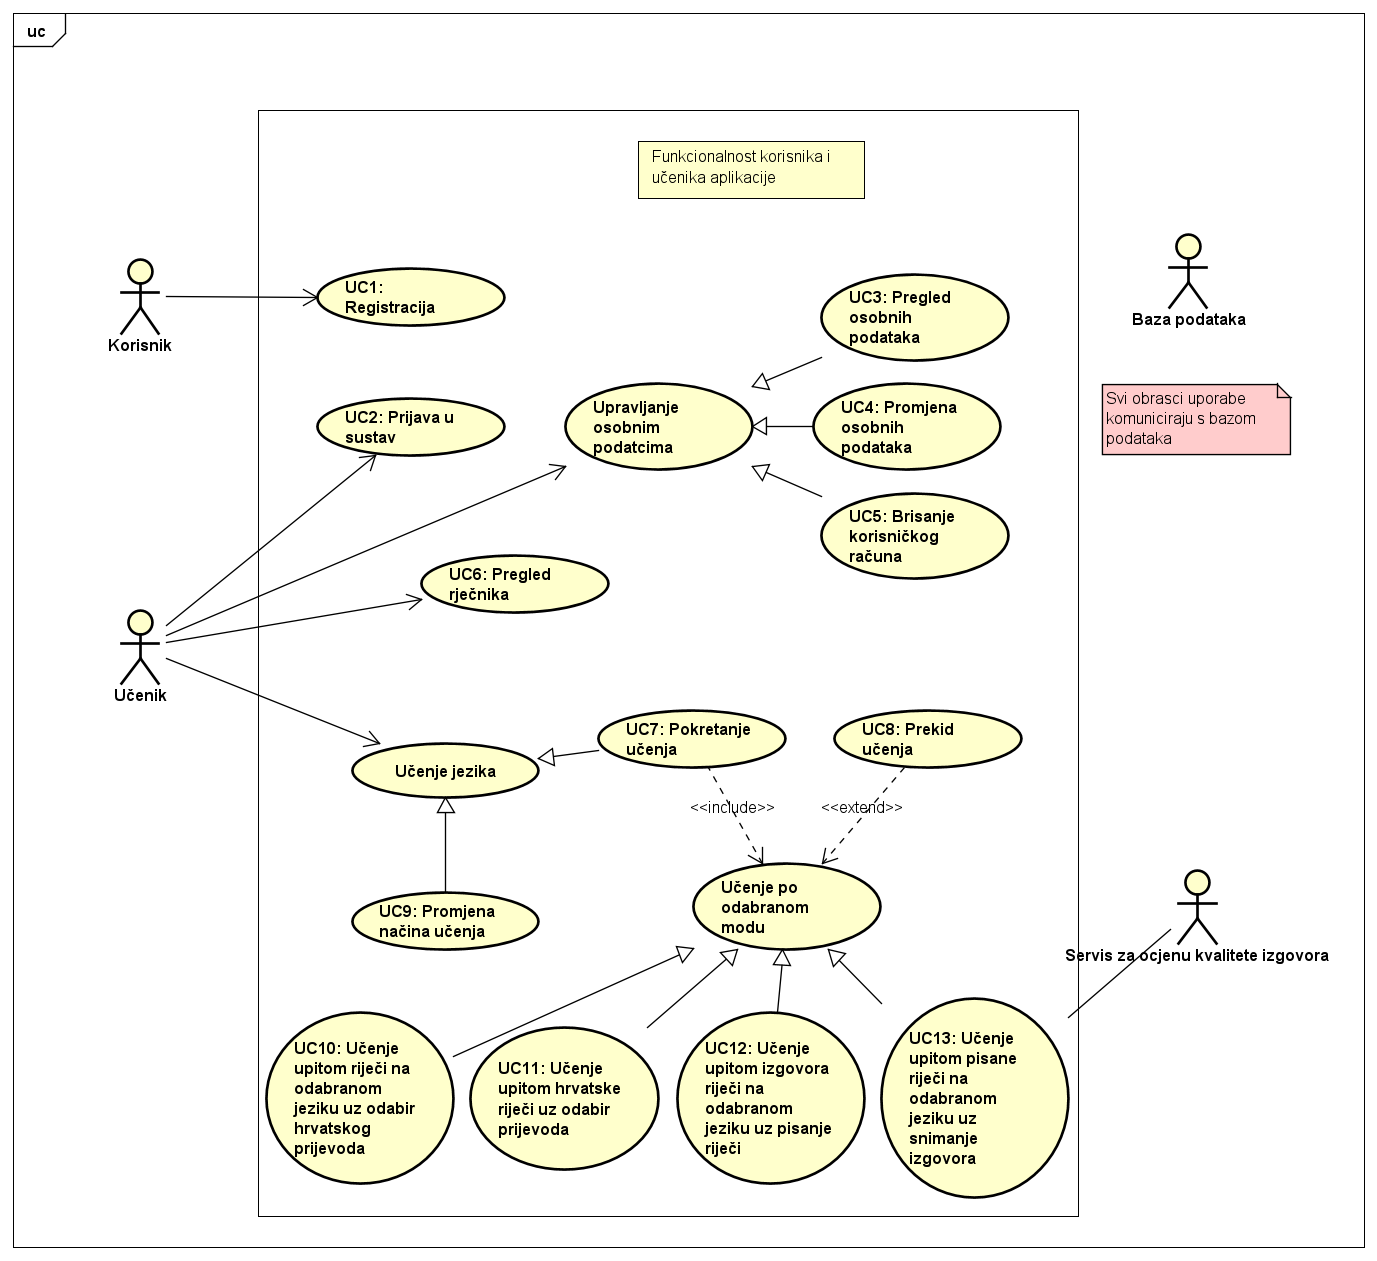
\includegraphics[width=\textwidth]{dijagrami/ucdiag1.png} %veličina u odnosu na širinu linije
						\caption{Dijagram obrasca uporabe, funkcionalnost korisnika i učenika}
						\label{fig:ucdiag1} %label mora biti drugaciji za svaku sliku
					\end{figure}

					\begin{figure}[H]
						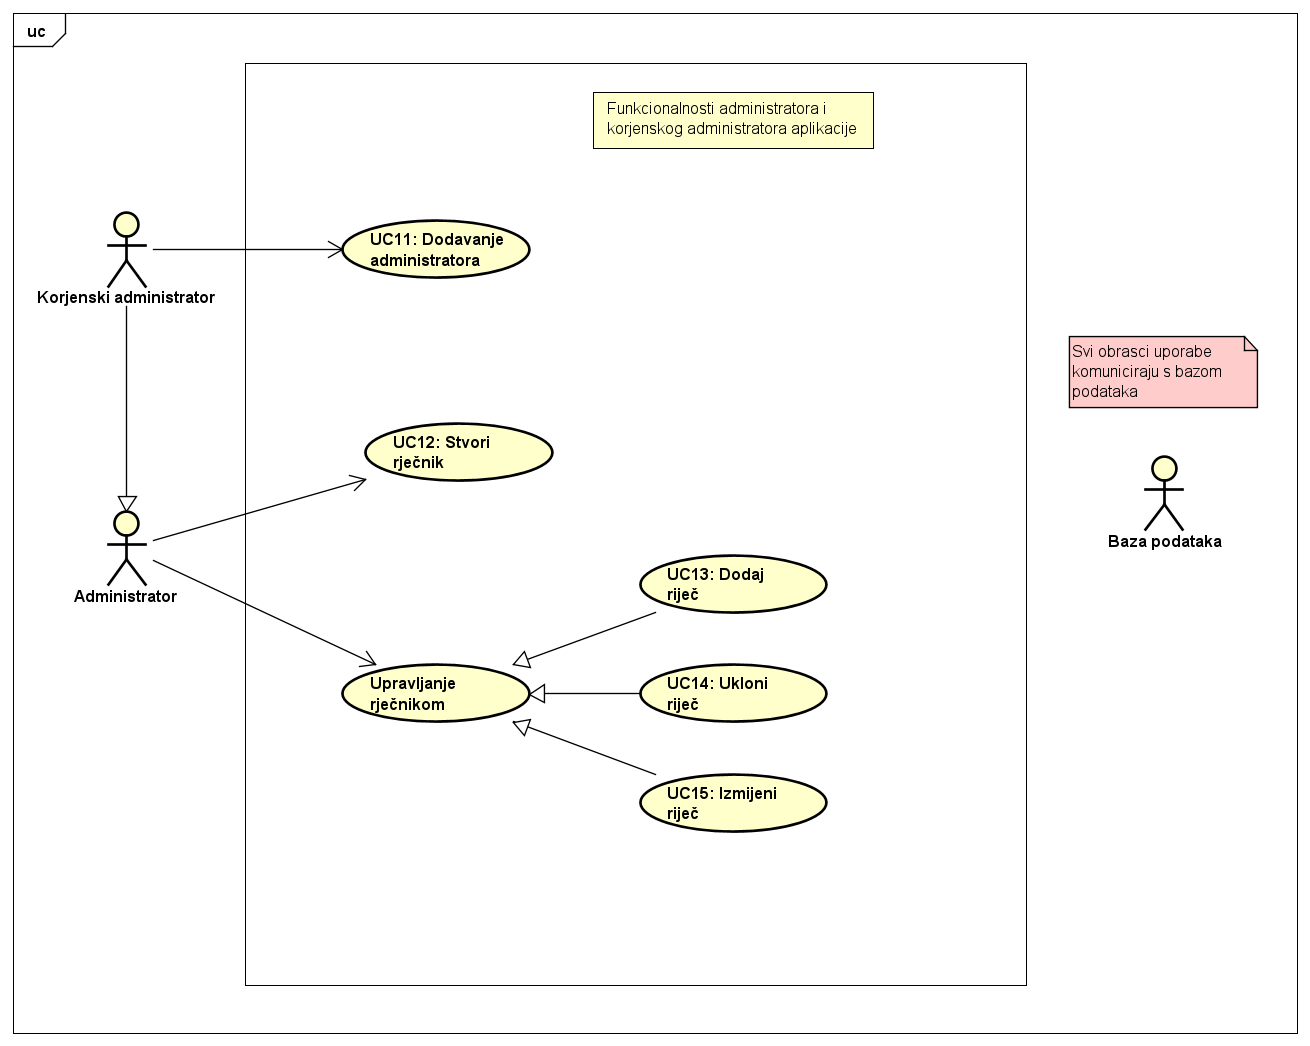
\includegraphics[width=\textwidth]{dijagrami/ucdiag2.png} %veličina u odnosu na širinu linije
						\caption{Dijagram obrasca uporabe, funkcionalnost korijenskog administratora i administratora}
						\label{fig:ucdiag2} %label mora biti drugaciji za svaku sliku
					\end{figure}

				\eject		
				
			\subsection{Sekvencijski dijagrami}
				
				\textbf{\textit{dio 1. revizije}}\\
				
				\textit{Nacrtati sekvencijske dijagrame koji modeliraju najvažnije dijelove sustava (max. 4 dijagrama). Ukoliko postoji nedoumica oko odabira, razjasniti s asistentom. Uz svaki dijagram napisati detaljni opis dijagrama.}
				
				\subsubsection{Obrasci uporabe UC3 i UC4 - Osobni podatci}
                    Učenik je prijavljen u sustav. Odabire opciju "Osobni podatci" te dobiva listu osobnih podataka koje može mijenjati.
                    Može promijeniti svoje osobne podatke ako želi. Učenik mijenja svoje podatke te pokušava izaći iz "Osobnih podataka".
                    Sustav ga obavještava da pokušava izići bez spremanja promjena te ga pita želi li nastaviti tako ili želi spremiti svoje promjene.
                    Nakon odabira baza podataka ažurira osobne podatke.

                    \begin{figure}[H]
                        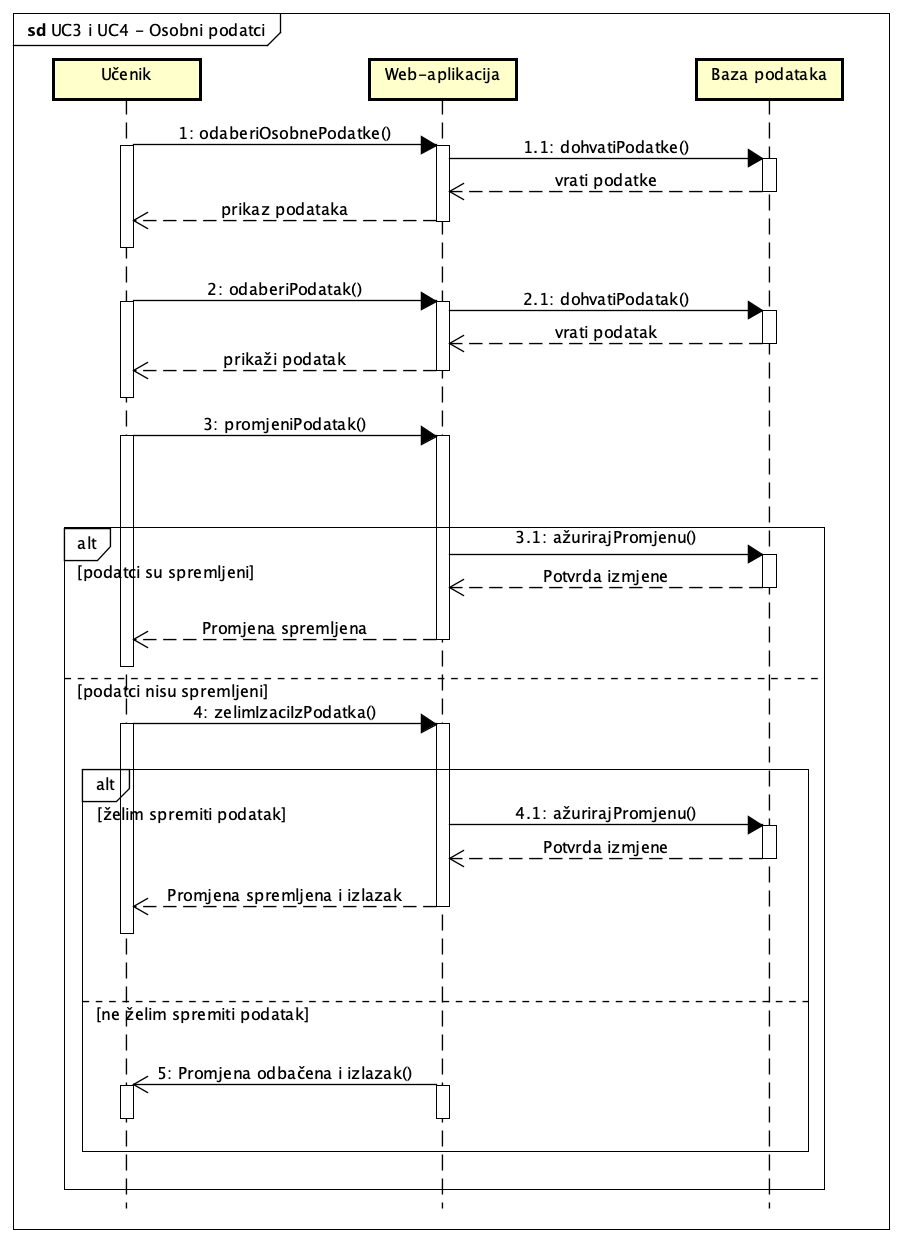
\includegraphics[width=\textwidth]{dijagrami/sdiag1.png}
                        \caption{Sekvencijski dijagram osobnih podataka}
                        \label{fig:sdiag1}
                    \end{figure}

                \eject

				\subsubsection{Obrasci uporabe UC16, UC17 i UC18 - Dodaj, ukloni i izmjeni riječi}
					Korisnik je prijavljen u sustav. Dobio je administratorska prava. Administrator ima tri moguće opcije.
					Odabire dodavanje riječi. Zatim dobiva popis jezika i rječnike koje može odabrati i u njih dodati riječ.
					Upisuje riječ koju želi dodati. Moguće je da već postoji upisana riječ u rječniku te sustav obavještava administratora
					da modificira upisanu riječ ili da napiše novu riječ. Nakon toga pokreće se pretraga na vanjskom rječniku. 
					Administrator odabire opis i podatke bitne za riječ koje je dobio od vanjskog rječnika. Uređuje podatke te potvrđuje 
					njihov unos te nakon toga baza podataka ažurira riječ za odabrani jezik i rječnik. Druga opcija je uklanjanje riječi
					te odabire tu opciju. Dobiva popis jezika i rječnika koje može odabrati. Odabire jezik i rječnik. Upisuje riječ koju
					želi ukloniti. Sada postoji mogućnost da riječ koju je upisao ne postoji u rječniku te da upiše novu riječ. Nakon upisane
					ispravne riječi ta riječ se uklanje iz tog rječnika i jezika te se ažurira baza podataka prema tome. Treća opcija koju može
					odabrati je izmjena riječi. Dobiva popis jezika i rječnika koje može odabrati. Nakon odabira dobiva mogućnost upisa riječi
					koju želi izmjeniti. Upisuje željenu riječ. Moguće je da upisana riječ ne postoji u rječniku te sustav obavještava administratora
					da modificira riječ ili upiše novu. Nakon upisa ispravne riječi dobiva opis i podatke te riječi koje može promjeniti.
					Mijenja njene podatke. Tada može spremiti podatke ili ih može zaboraviti spremiti te ga u tom trenutku obavještava sustav 
					da nije spremio izmjene te želi li nastaviti ili spremiti izmjene. Nakon toga se ažurira baza podataka.

					\begin{figure}[H]
						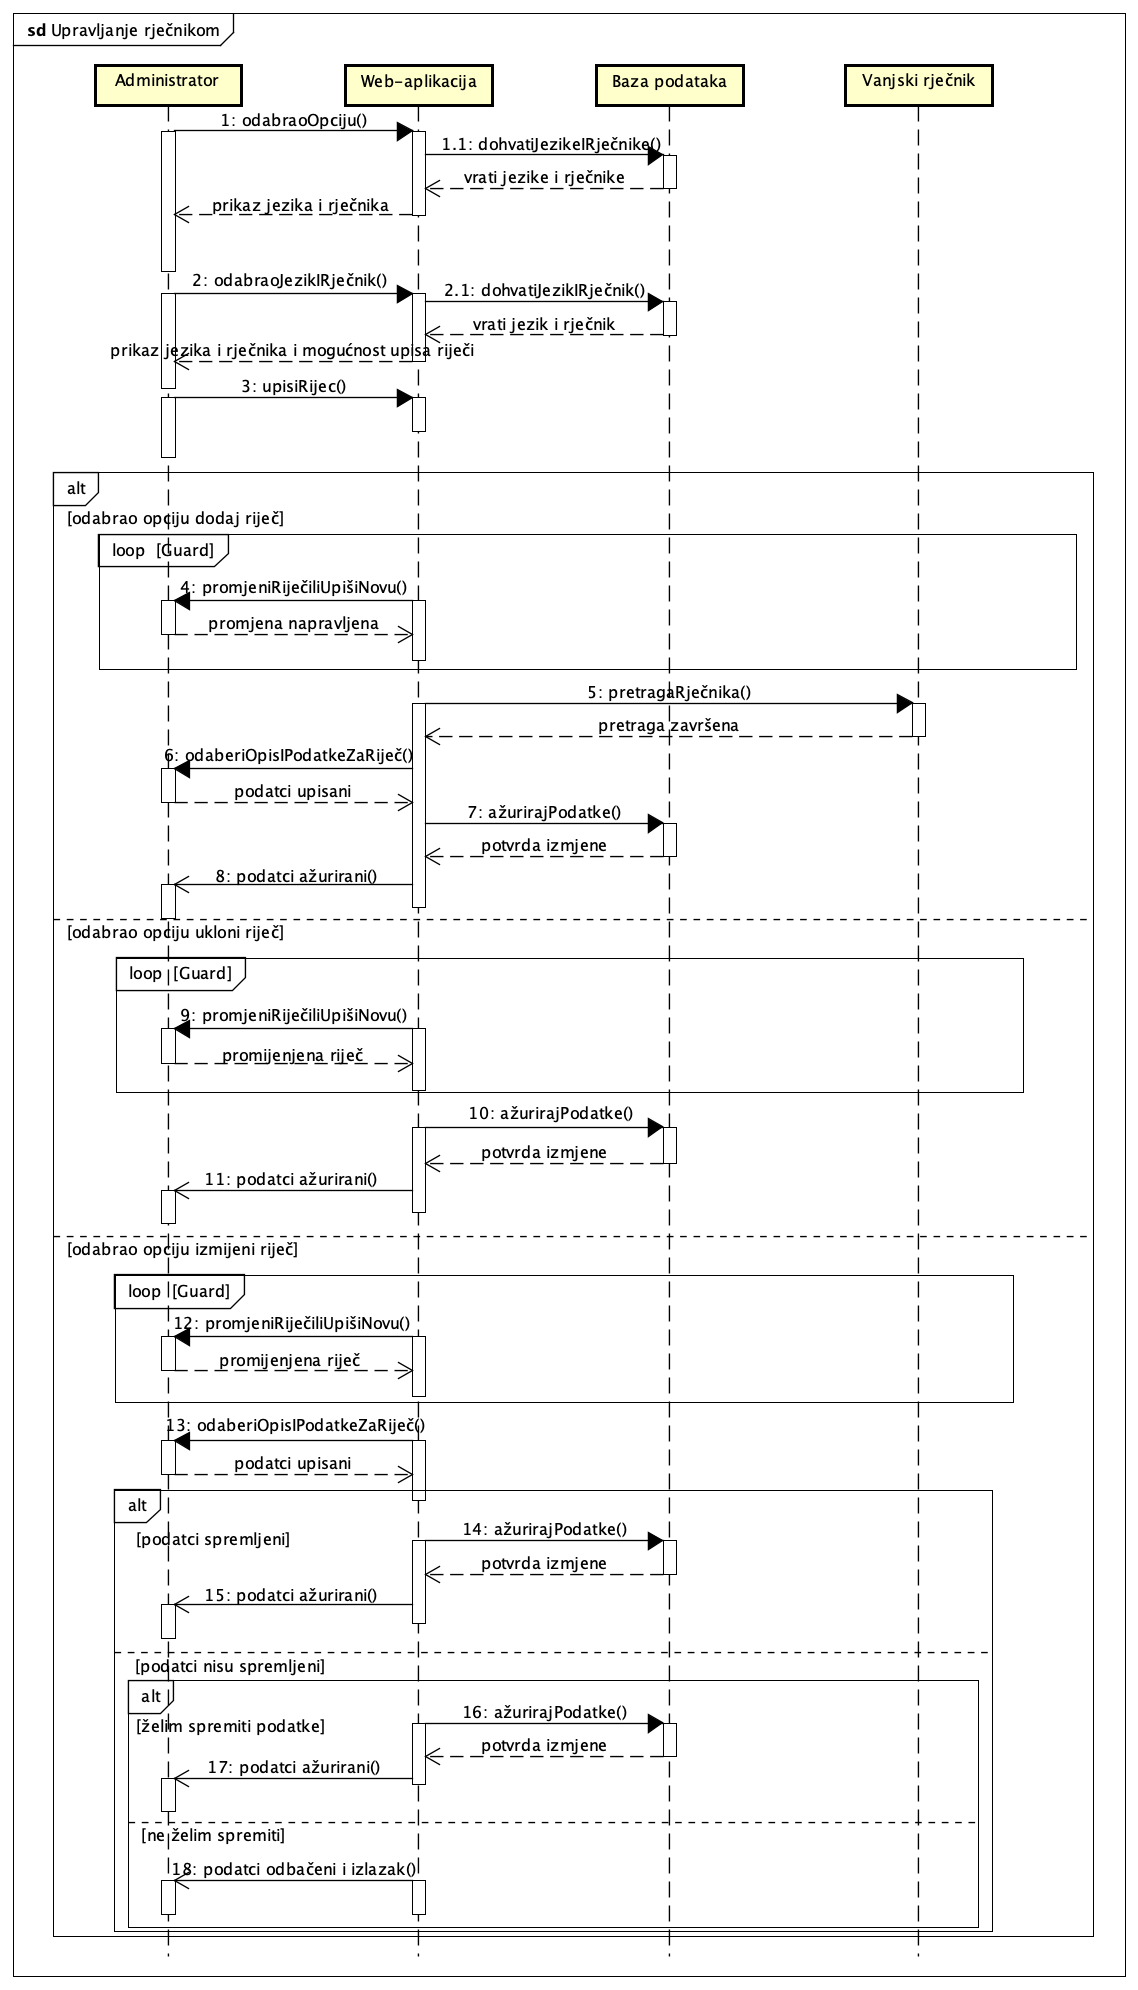
\includegraphics[width=\textwidth]{dijagrami/sdiag2.png}
						\caption{Sekvencijski dijagram upravljanja rječnikom}
						\label{fig:sdiag2}
					\end{figure}

				\eject	

			\eject
	
		\section{Ostali zahtjevi}
		
			\textbf{\textit{dio 1. revizije}}\\
		 
			 \textit{Nefunkcionalni zahtjevi i zahtjevi domene primjene dopunjuju funkcionalne zahtjeve. Oni opisuju \textbf{kako se sustav treba ponašati} i koja \textbf{ograničenja} treba poštivati (performanse, korisničko iskustvo, pouzdanost, standardi kvalitete, sigurnost...). Primjeri takvih zahtjeva u Vašem projektu mogu biti: podržani jezici korisničkog sučelja, vrijeme odziva, najveći mogući podržani broj korisnika, podržane web/mobilne platforme, razina zaštite (protokoli komunikacije, kriptiranje...)... Svaki takav zahtjev potrebno je navesti u jednoj ili dvije rečenice.}
			 
			 
			 
	